\documentclass{standalone}

\usepackage{tikz}
\usetikzlibrary{scopes}
\begin{document}

\def\iangle{35} % Angle of the inclined plane

\def\down{-90}
\def\arcr{0.5cm} % Radius of the arc used to indicate angles

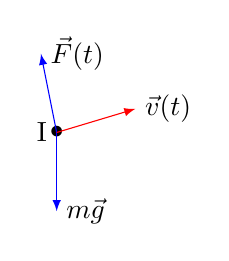
\begin{tikzpicture}[
    force/.style={>=latex,draw=blue,fill=blue},
    cine/.style={>=latex,draw=red,fill=red},
    axis/.style={densely dashed,gray,font=\small},
    M/.style={rectangle,draw,fill=lightgray,minimum size=0.5cm,thin},
    m/.style={circle,draw=black,fill=lightgray,minimum size=0.03cm,thin},
    plane/.style={draw=black,fill=blue!10},
    string/.style={draw=red, thick},
    pulley/.style={thick},
]


    %%%
    % Free body diagram of m
    %\node[m] (m) {};
    \coordinate (I) at (0, 0);
    \draw(I) node{$\bullet$};
    \draw (I)node[left]{I};
    {[force,->]
        \draw (I.north) -- ++(-0.2,1) node[right] {$\vec{F}(t)$};
        \draw (I.south) -- ++(0,-1) node[right] {$m\vec{g}$};
    }
    {[cine,->]
        \draw (I.east) -- ++(1,0.3) node[right] {$\vec{v}(t)$};
    }

\end{tikzpicture}

\end{document}
